\section{Method}

\begin{figure}[htp]
    \centering
    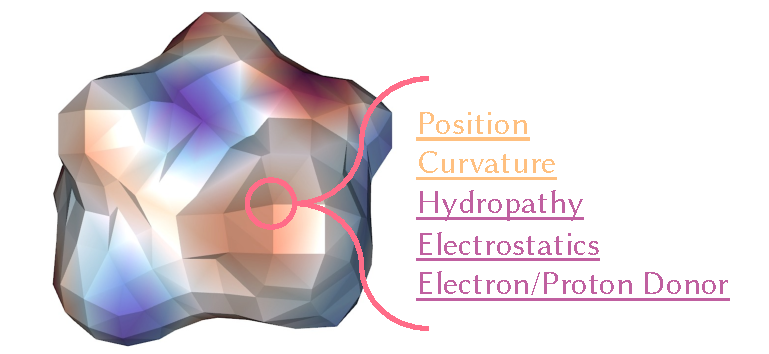
\includegraphics[width=0.5\linewidth]{figures/features.pdf}
    \caption{
        During the data pre-processing phase, we assign each vertex to the molecule's solvent-accessible surface area (SASA) with a total of five features: two geometrical (orange) and three chemical (purple) features.
        Some of these features are then decomposed by the Laplace-Beltrami operator to further exploit the intrinsic geometric and chemical properties of the molecular surface.
    }
    \label{fig:feature}
\end{figure}

Here we outline our data pre-processing approach, particularly emphasizing the computation of features on the molecule's solvent-accessible surface area.

\subsection{Data Pre-processing}

\paragraph{Solvent Accessible Surface}
The solvent-accessible surface area (SASA) describes the water-tight surface area of a biomolecule that is accessible to a solvent.
The solvent-accessible surface area (SASA) is depicted by the center of a solvent molecule, often modeled as a sphere (like a water molecule), as it traverses the surface of the biomolecule.
We use the \texttt{MSMS} \cite{MSMS} software that converts PDB in the point cloud format into the SAS in mesh format.

\paragraph{Features of Molecule}
The SASA of a molecule provides positional information, but this alone is insufficient for thorough network learning. To achieve a comprehensive understanding, it's essential to incorporate both geometric and chemical features in MaSIF\cite{MaSIF}.

For every vertex of the SASA, we attribute two geometric characteristics (position and curvature) and three chemical attributes (hydropathy index, continuum electrostatics, and the positions of free electrons and proton donors) to it, as depicted in Figure\ref{fig:feature}.

\paragraph{Geometric Features}
The position of each vertex has already been stored in the SASA.
Based on the mesh data, we use the libigl package to calculate the mean and Gaussian curvatures, which are then transformed to the principal curvatures, denoted as $\kappa_1$ and $\kappa_2$ with $\kappa_1>\kappa_2$.
Following MaSIF \cite{MaSIF}, these principal curvatures are then transformed to a range of $(-1, 1)$ with following formula
\begin{equation}
    \frac{2}{\pi}\arctan\frac{\kappa_1+\kappa_2}{\kappa_1-\kappa_2}
\end{equation}
where $-1$ denotes the most concave and $1$ the most convex.

\paragraph{Chemical Features}
We obtain each chemical feature from previous works and relevant software. For the hydropathy index, we consult Kyte and Doolittle's scale table for the 20 amino acid side chains \cite{hydropathy}.
For the continuum electrostatics, we use \texttt{PDB2PQR} \cite{PDB2PQR} to add hydrogen atoms to protein structures in PDB format.
Then, we use \texttt{APBS} \cite{APBS} to calculate the Poisson–Boltzmann electrostatics for each protein.

For the location of free electrons and proton donors, we follow the methodology derived from MaSIF\cite{MaSIF}, which assigns each vertex a value based on its proximity to the nearest heavy atom.

\begin{figure*}
    \centering
    % 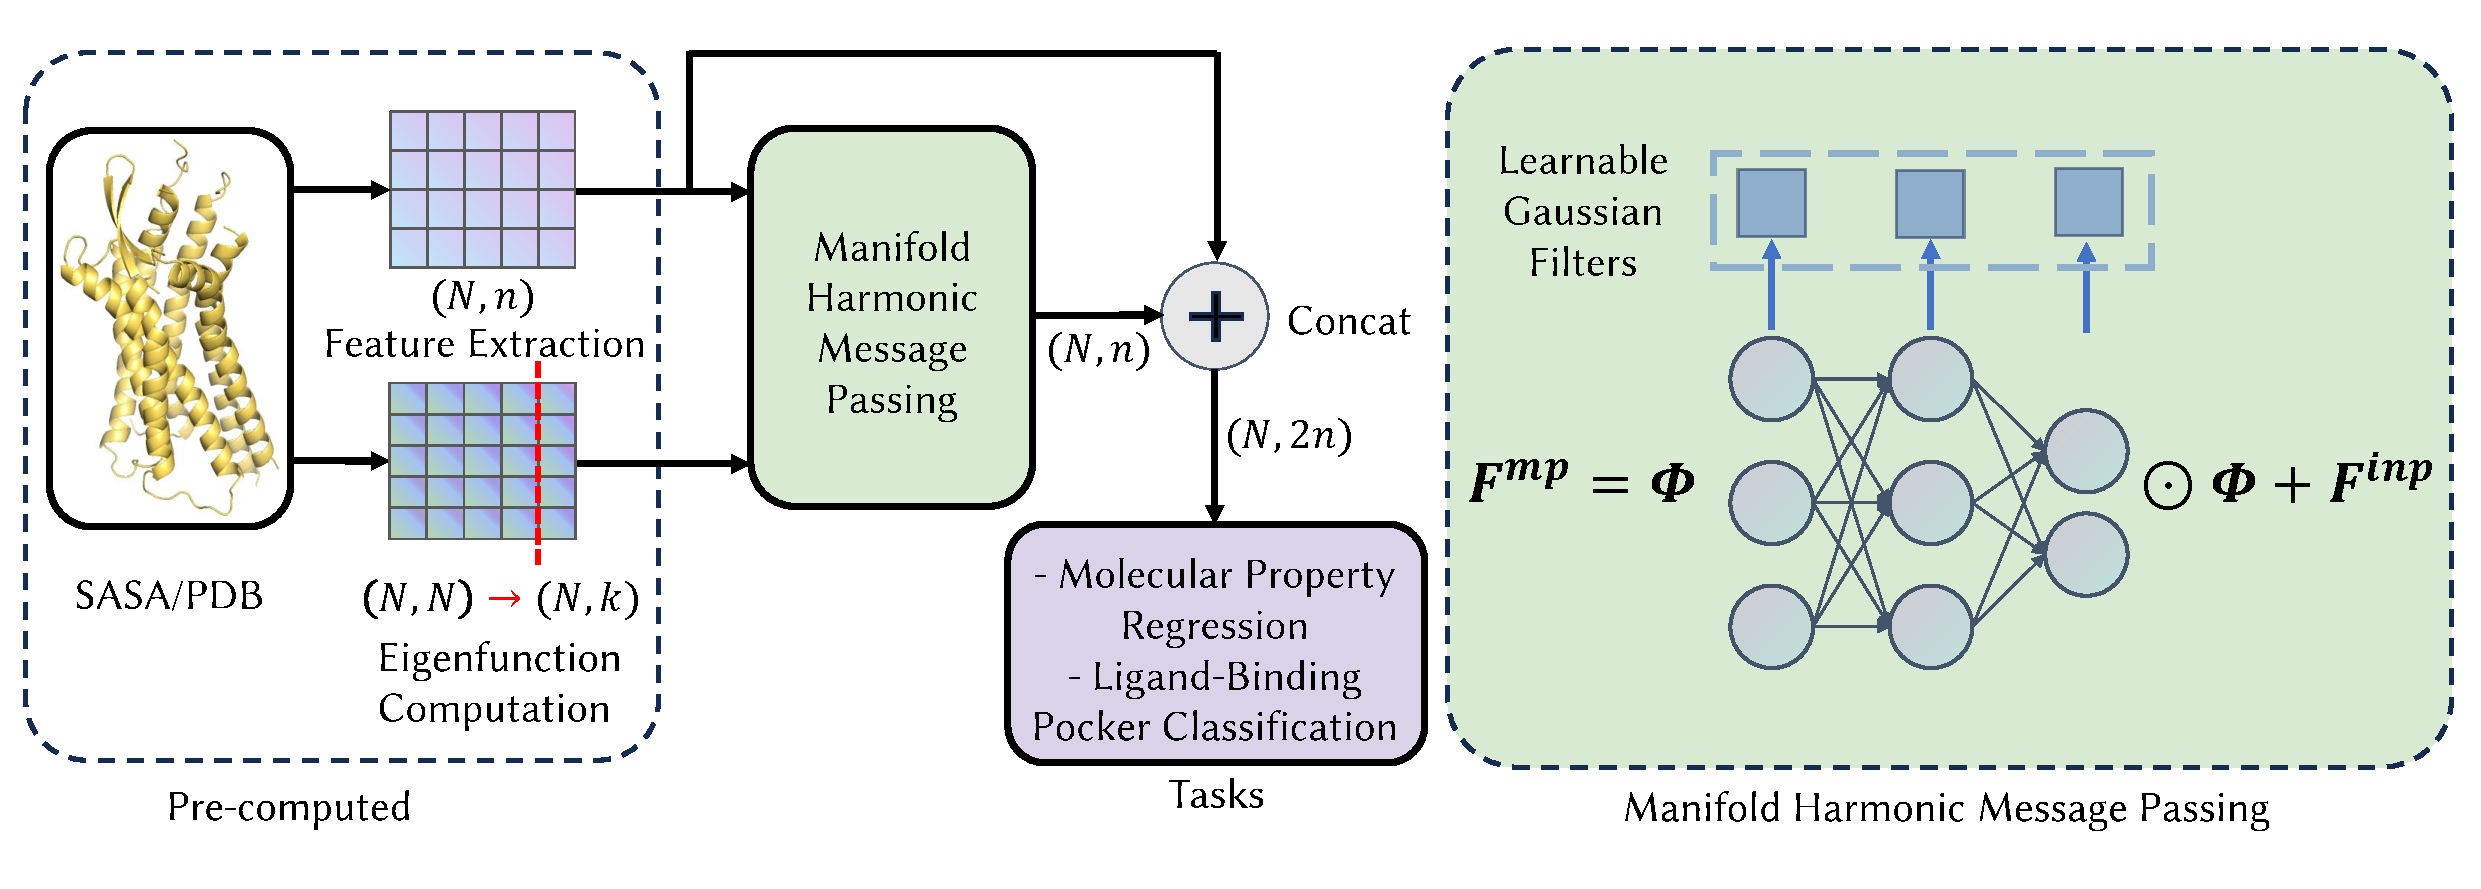
\includegraphics[width=\linewidth]{figures/pipeline.pdf}
    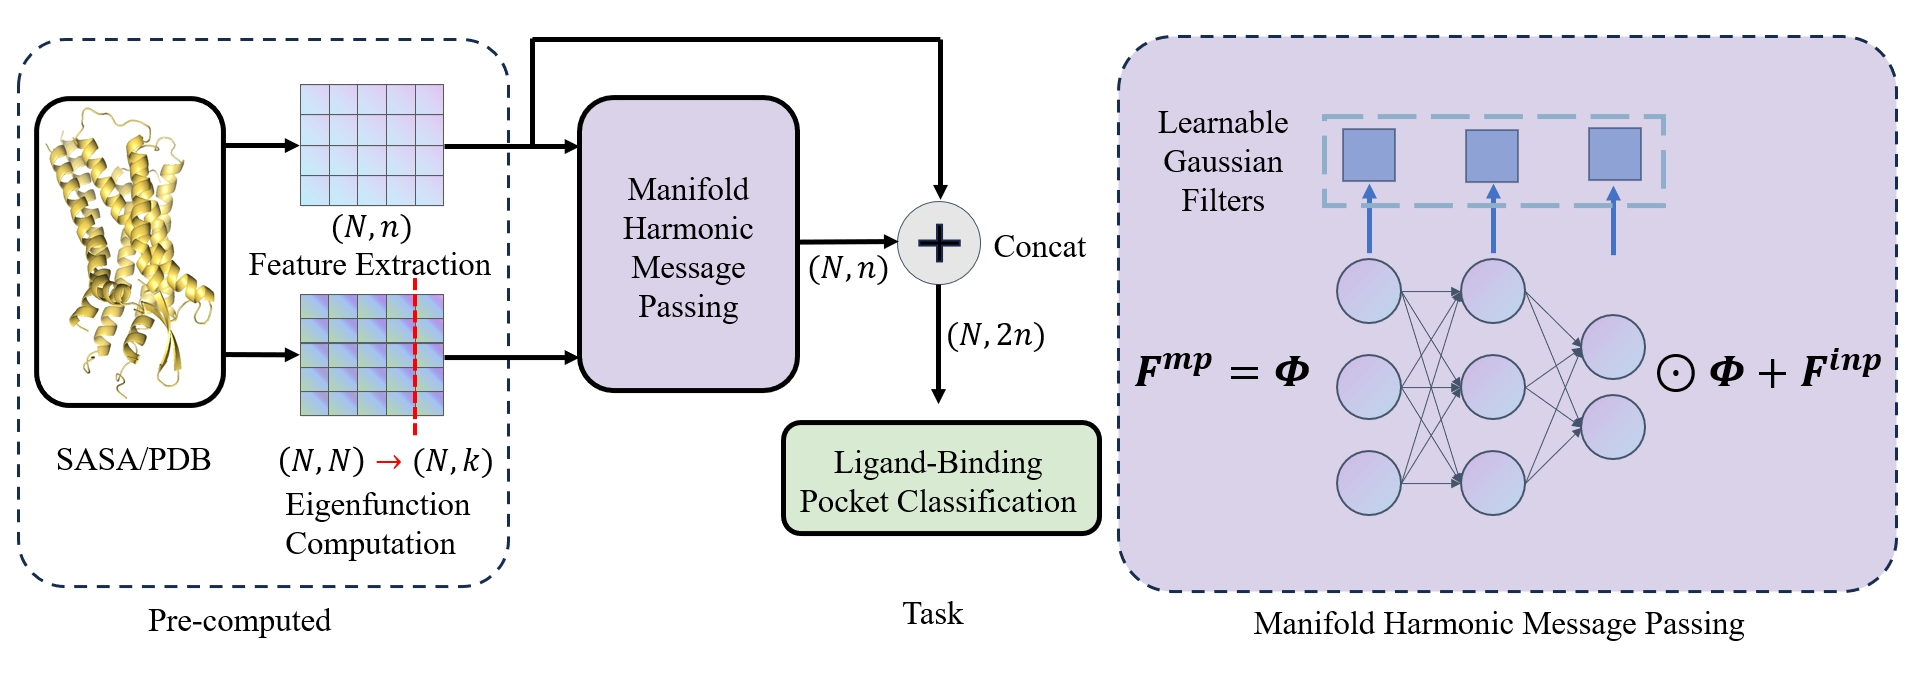
\includegraphics[width=\linewidth]{figures/pipeline.jpg}
    \caption{
        Pipeline.
        Given a protein surface SASA with $N$ vertices, we keep the first $k$ Laplace-Beltrami eigenfunctions with the truncated ascending eigenvalues.
        Then these eigenfunctions are sent into the Manifold Harmonic Message Passing module, which is primarily a fully connected network with the Heat Kernel Signatures.
        The output of the Manifold Harmonic Message Passing module is concatenated with features and sent to the downstream tasks, such as ligand-binding pocket classification.
    }
    \label{fig:pipeline}
\end{figure*}

\subsection{Laplace–Beltrami Decomposition}

To further exploit the features of the molecule's SASA, we apply the Laplace–Beltrami decomposition technique.
Intuitively, each feature is treated as a continuous real-valued function defined on the SASA, which is akin to a 2D manifold.
Similar to the Fourier transform, utilizing a series of orthonormal basis functions, denoted as $\{\phi_i\}$, to decompose the target function.
The basis functions are defined by the equation:
\begin{equation}
    \Delta\phi_i=\lambda_i\phi_i
\end{equation}
where $\Delta=-\nabla\cdot\nabla$ represents the Laplacian operator defined on the manifold.
$\lambda_i$ is the corresponding eigenvalue of $\phi_i$ arranged in ascending order, that is, $0\le\lambda_0\le\lambda_1\le\cdots$.
Figure \ref{fig:Laplace-Beltrami} shows the Laplace-Beltrami decomposition of the electrostatics field defined on a protein surface.

For a discrete surface mesh with $N$ vertices, the application of the Laplace-Beltrami decomposition results in the generation of $N$ eigenfunctions,
Each of these consists of $N$ values.
Therefore, this process yields a $N\times N$ eigenfunction matrix and $N\times 1$ eigenvalue matrix.
However, the complete utilization of this matrix significantly escalates computational costs.

To optimize this, a common strategy is to keep only the first $k$ eigenfunctions.
In our method, $k$ is selected differently for each downstream task.
The Laplace-Beltrami decomposition is done by \texttt{scipy}, following \texttt{HMR} \cite{HMR}.

We then transform the retained eigenfunctions and eigenvalues into the input for the downstream task, that is, ligand-binding pocket classification, using a fully connected network are concatenated with features extracted in the previous stage, as illustrated in figure \ref{fig:pipeline}.